\section{Kritische Würdigung}

\subsubsection*{Versuchsdurchführung}

Für die dritte Mode haben wir offensichtlich leider den falschen Messbereich ausgewählt.
Was wir als Resonanzkurve vermuteten, stellt sich als Artefakt heraus.
Für höhere Temperaturen \enquote{wandert} die tatsächliche Resonanzkurve in Richtung Null, sodass sie teilweise im Messbereich noch dargestellt wird.

Man erkennt dies außerdem gut im Plot der über die Temperatur aufgetragenenen Resonanzfrequenzen:
Was die Fehler der Messpunkte in y-Richtung (also der Fehler auf $\omega_R$) angeht, haben alle Punkte relativ kleine Fehler - die Fehlerbalken sind nahezu nicht sichtbar.
Für die dritte Mode erkennt man für die erste Hälfte der Messwerte (im kälteren Temperaturbereich also) jedoch deutlich größere Fehler.
Hier war der Fit einfach nicht sehr erfolgreich aufgrund der unklaren Messpunkte.
Je wärmer, desto besser werden die Fehler: die Kurve \enquote{wandert} in den Messbereich und sorgt für bessere Fits.

\subsubsection*{Einordnung der Fiteigenschaften}

Beim Erstellen der Fits an die aufgenommenen Daten geht es uns darum, das in der Einleitung beschriebene theoretische Modell möglichst gut an die aufgenommenen Daten anzupassen.
Daraus können wir zum einen schließen, ob das Modell die Realität tatsächlich beschreibt - und zum anderen erhalten wir so auch weitere Informationen über das System:
Wir können etwa die Resonanzfrequenzen der Schwingung genau feststellen.

Letzteres funktioniert sehr gut.
Die Fehler auf $\omega_0$ sind winzig.
Dies liegt allerdings zu großen Teilen am verwendeten Mittleren Fehler auf den Mittelwert der Messungen.
Die große Anzahl an Einzelmessungen lässt den Fehler auf die Messpunkte verschwindend gering werden.

Für $\omega_{0}$ passt die Lorentzkurve sehr gut an die Daten.
Dies ist in den Plots ersichtlich und wird auch durch den guten $\chi_{red}^2$-Wert belegt.
Dennoch liegt die Fitwahrscheinlichkeit nur bei unter 10\%.

\subsubsection*{Vergleich mit den theoretischen Verhältnissen}

In der Einleitung Gleichung \ref{eq:VerhaeltnisseEigenfrequenzen} wurden theoretische Verhältnisse der Eigenfrequenzen $\frac{\nu_1}{\nu_0}$ und $\frac{\nu_2}{\nu_0}$ eingeführt.
Diese Werte lassen sich nun mit den von uns gewonnenen experimentellen Ergebnissen vergleichen.
Die Ergebnisse sind in Tabelle \ref{tab:VergleichEigenfrequenzen} aufgetragen.

\minipage{\linewidth}
    \begin{center}
        \captionsetup{type=table}
        \begin{adjustbox}{max width=\linewidth, keepaspectratio}
            \begin{tabular}{llllll}
            \toprule
            $\left ( \frac{\nu_1}{\nu_0} \right )_{theo}$ & $\left ( \frac{\nu_1}{\nu_0} \right )_{exp}$ & Abweichung & $\left ( \frac{\nu_2}{\nu_0} \right )_{theo}$ & $\left ( \frac{\nu_2}{\nu_0} \right )_{exp}$ & Abweichung \\
            \midrule
            6.267 & 6.22590 $\pm$ 0.00016 & 0.041 $\overset{\wedge}{=}$ 260 $\sigma$ & 17.548 & 17.620 $\pm$ 0.098 & 0.072 $\overset{\wedge}{=}$ 0.73 $\sigma$ \\
            \bottomrule
            \end{tabular}
        \end{adjustbox}
        \captionof{table}{Vergleich von experimentellen und theoretischen Verhältnissen zwischen den Eigenfrequenzen}
        \label{tab:VergleichEigenfrequenzen}
    \end{center}
\endminipage

Wir erkennen für $\frac{\nu_1}{\nu_0}$ eine große Abweichung von 260 $\sigma$.
Diese ist allerdings damit zu begründen, dass die Fehler $\omega_0$ der einzelnen Moden so gering sind.
Die relative Abweichung mit $\frac{0.041}{6.267} = 0.7\%$ ist nicht besonders groß und so kann davon ausgegangen werden, dass die Eigenfrequenzen tatsächlich gefunden wurden.

\subsubsection*{Interpretation der Abschätzung systematischer Fehler}

Wir betrachten die residuals in den Abbildungen der Amplituden.
Es wird deutlich, dass zu keiner der Resonanzfrequenzen erhebliche Trends von systematischen Abweichungen im Messbereich sichtbar sind.

\subsubsection*{Vergleich der berechneten Güte für die erste Mode}

Wir haben die Daten der Amplitude $A$ verwendet und einerseits mit den aus dem Fit gewonnenen Parametern die Güte $Q_{Fit} = 59.06 \pm 0.19$ errechnet.
Andererseits haben wir die full width (FW) auf der Höhe des $\frac{1}{\sqrt{2}}$-fachen Maximums der Lorentzkurve zu $FW = \SI{34}{\second^{-1}}$ bestimmt und anschließend die Güte
\begin{align}
    Q_{FW} = \frac{\omega_R}{FW} = 59.05
\end{align}

berechnet. Da nur ein qualitativer Vergleich angestellt werden soll, verzichten wir an dieser Stelle auf die Abschätzung eines Fehlers für $Q_{FW}$.

Die oben genannten Werte bedeuten eine Abweichung von $Q_{FW}$ zu $Q_{Fit}$ um \SI{0.01} absolut - beziehungsweise \SI{0.05}{\sigma}.
Wir können also davon ausgehen, dass die Bestimmung der Güte mit beiden Methoden gleich gut funktioniert - je nachdem, welche Methode sich gerade besser anbietet.

\subsubsection*{Temperaturabhängigkeit der Resonanzfrequenzen}

In den Abbildungen \ref{fig:Temperaturabhaengigkeit0}, \ref{fig:Temperaturabhaengigkeit1} und \ref{fig:Temperaturabhaengigkeit2} erkennen wir eine negative Steigung der Temperaturabhängigkeit der Resonanzfrequenzen.
Das bedeutet, dass bei höheren Temperaturen die Resonanzfrequenz abnimmt.

Mit Gleichung \ref{eq:TransversaleAuslenkung} sehen wir, dass sich dieses Verhalten auf die Temperaturabhängigkeit der Schallgeschwindigkeit im Reed zurückführen lässt.
Je höher die Temperatur im Festkörper, desto geringer wird die Schallgeschwindigkeit.
Dies ist anders als zum Beispiel bei idealen Gasen.

Dabei stellen wir zudem fest, dass sich die Temperaturabhängigkeit für die verschiedenen Moden unterscheidet.

\subsubsection*{Analyse möglicher Fehlerquellen}

In dem verwendeten Versuchsaufbau gibt es eine Vielzahl von möglichen systematischen Fehlerquellen.
Einige intuitive Störungen wie beispielsweise Luftreibung der Schwingung haben nur eine vernachlässigbare Auswirkung auf das Resonanzverhalten des Reeds.
Hingegen beeinflussen Faktoren wie schräges Einspannen oder Mitschwingen der Einspannungen das Schwingverhalten des Systems stark.
Als Folge lässt sich die Schwingung des Reeds nicht mehr durch die verwendete Theorie beschreiben.
Die Größte solcher Fehler lässt sich nur schwer abschätzen.
Wie wir allerdings festgestellt haben, sind die absoluten Abweichungen der Frequenzverhältnisse im Bereich weniger Prozent.

\subsubsection*{Python/PyVISA als Alternative zu LabVIEW}

Es stellt sich während der Durchführung dieses Versuchs heraus, dass die meiste Zeit nicht dafür verwendet wird, einen passenden Algorithmus für die Messung zu finden - sondern damit, das passende LabVIEW Modul zu finden.
Da der Titel dieses Versuchs nicht \enquote{Computeransteuerung und Datenverarbeitung mit LabVIEW} lautet, sind wir darüber doch ein Stück weit enttäuscht.
Auf der einen Seite haben wir LabVIEW kennengelernt - auf der anderen Seite war der Lerneffekt dieses Versuchs während der Durchführung fast ausschließlich darauf beschränkt.
(Die spätere Auswertung des Versuchs durch die statistische Analyse beziehungsweise den Fits sei unabhängig davon zu betrachten - dabei haben wir zusätzlich neue Methoden kennengelernt.)

Aus diesem Grund wäre es schön, umfangreichere Messmethoden zu verwenden, um dem Aspekt \enquote{Computeransteuerung} des Versuchs gerecht zu werden.
Dabei schließt es sich selbstverständlich nicht aus, dass zum Kennenlernen erste, einführende Messungen mit LabVIEW durchgeführt werden - das grundlegende Prinzip und die Vorteile von LabVIEW sind schnell verstanden.
Es wäre allerdings möglich, dass die anschließenden, ausführlicheren Messalgorithmen dann nicht in Kleinstarbeit mit LabVIEW geskriptet werden, sondern in Python implementiert werden können.
Das PyVISA Modul für Python stellt eine Schnittstelle zu VISA beziehungsweise schließlich zum GPIB dar.
Es können also alle Geräte dieses Versuchs mit Python-Code angesprochen und gesteuert werden.
Python wird bereits im Anfänger-Praktikum für viele Versuchsauswertungen verwendet und ist daher in Grundlagen allen Studierenden bekannt.

Unser gesamtes LabVIEW-Skript der Messung, wie in Abbildung \ref{fig:LabVIEWSkript} dargestellt, lässt sich auf weniger als 30 Zeilen Python-Code verkürzen.

Leider ließ sich während unserer Durchführung des Versuchs auf den Praktikumsrechnern aufgrund veralteter Software das PyVISA Modul nicht installieren.
Als beispielhafte Alternative haben wir stattdessen Teile des Versuchs mit PyVISA simuliert.

\subsubsection*{Simulation des Versuchs}

In \texttt{measure.py} steht der Python-Code für eine beispielhafte Messung im Frequenzbereich rund um die erste Mode.
Zunächst bauen wir eine GPIB-Verbindung zum Frequenzgenerator unter Adresse 19 beziehungsweise zum Lock-In-Verstärker unter Adresse 7 auf:
\begin{small}
\begin{lstlisting}[xleftmargin=10mm,numbers=none]
self.frequency_generator = rm.open_resource("GPIB::19")
self.lock_in_amplifier = rm.open_resource("GPIB::7")
\end{lstlisting}
\end{small}

Mit
\begin{small}
\begin{lstlisting}[xleftmargin=10mm,numbers=none]
frequencies = np.linspace(158, 162, 200)
\end{lstlisting}
\end{small}

bestimmen wir 200 Messpunkte mit Frequenzen am Generator von \SIrange{158}{162}{\hertz}. Wir setzen die Frequenz am Generator
\begin{small}
\begin{lstlisting}[xleftmargin=10mm,numbers=none]
self.frequency_generator.query("FREQ {:f}".format(f))
\end{lstlisting}
\end{small}

und lesen die Werte für X- beziehungsweise Y-Kanal des Lock-In-Verstärkers aus
\begin{small}
\begin{lstlisting}[xleftmargin=10mm,numbers=none]
X = self.lock_in_amplifier.query("QX")
Y = self.lock_in_amplifier.query("QY")
\end{lstlisting}
\end{small}

Die dabei verwendeten GPIB-Befehle entsprechen den bereits aus der Versuchsanleitung \cite{Anleitung} bekannten Befehlen \texttt{FREQ}, \texttt{QX} und \texttt{QY}.
Die Wartezeit
\begin{small}
\begin{lstlisting}[xleftmargin=10mm,numbers=none]
idle_time = 50 / 1000
\end{lstlisting}
\end{small}

zwischen den Messungen ist für die Zwecke der Simulation ausreichend gering gewählt um keine unnötigen Verzögerungen zu produzieren.
Für tatsächliche Messungen kann (und sollte) dieser Wert entsprechend erhöht werden.

Anschließend werden die Messdaten in eine Datei geschrieben. Am Vergleich eines beispielhaften Auszugs dieser Datei
\begin{small}
\begin{lstlisting}[xleftmargin=10mm,numbers=none]
158.24120603015075 3.510229e-07 -3.856987e-08
\end{lstlisting}
\end{small}

mit einem Auszug aus der tatsächlichen Messdatei
\begin{small}
\begin{lstlisting}[xleftmargin=10mm,numbers=none]
1.110 158.900000 20.83E-6 44.08E-6
\end{lstlisting}
\end{small}

wird die Analogie im Aufbau zwischen simulierten und experimentell bestimmten Daten der beiden Messdateien deutlich.
Allein die erste Spalte der eingestellten Heizspannung am Peltier-Element fehlt.
(Der Aspekt der Temperaturabhängigkeit der Resonanzfrequenzen wird zur Zeit nicht untersucht, da diese Funktionalität der Simulation bisher von uns nicht implementiert wurde.)

Da - wie bereits erwähnt - keine \enquote{echte} GPIB-Verbindung besteht, können wir stattdessen mit PyVISA beziehungsweise PyVISA-sim die gesamte Kommunikation simulieren.
Wir definieren die beim Versuch verwendeten Geräte Funktionsgenerator und Lock-In-Verstärker in \texttt{devices.yml}.
Dabei geht es vor allem um die simulierten GPIB-Adressen und die unterstützten Befehle zum Setzen beziehungsweise Lesen der relevanten Werte.
Der Code von \texttt{simulate.py} läuft parallel zur Messung und speist die Geräte mit den passenden simulierten Daten.
Dabei haben wir uns an unseren experimentell bestimmten Werten für die erste Mode orientiert - diese sind aber selbstverändlich vollkommen frei wählbar.

Mit \texttt{plot.py} werden die simulierten Daten direkt einer ersten Auswertung unterzogen, indem Amplitude, Phase sowie X- und Y-Signal an die entsprechende Fitfunktion modelliert wird.
Ein beispielhaftes Ergebnis ist in Abbildung \ref{fig:PlotSimulation} zu sehen.

Der komplette Ablauf aus Messung, Simulation und Fit/Plot wird gestartet mit \texttt{main.py}.

\minipage{\linewidth}
    \begin{center}
        \captionsetup{type=figure}
        \begin{adjustbox}{max width=\linewidth, keepaspectratio}
            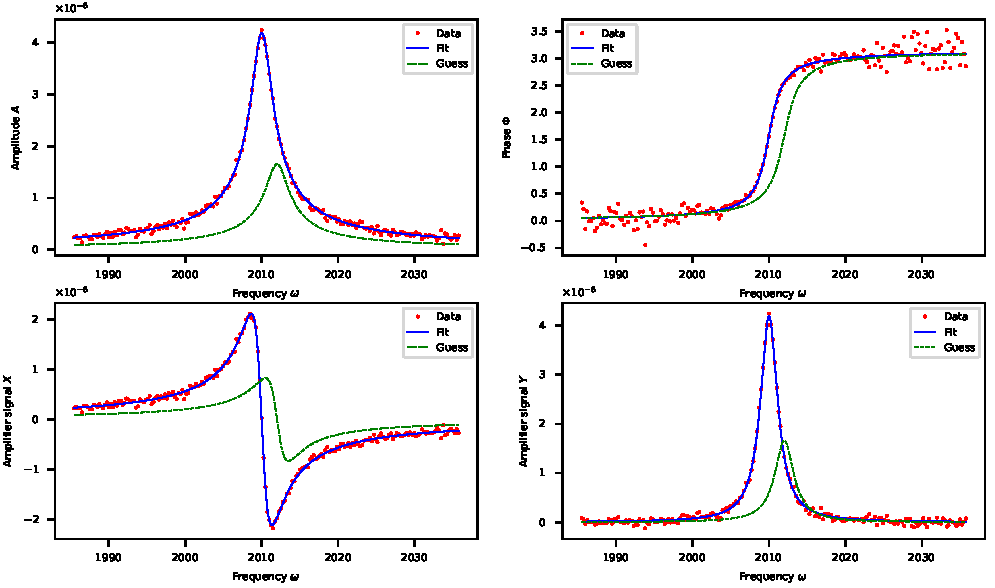
\includegraphics[]{pdf/Simulation}
        \end{adjustbox}
        \captionof{figure}{Beispielhafte Fit- und Plot-Ergebnisse für einen zufälligen Simulationsaufruf. Man erkennt die simulierten Messwerte inklusive ihrer Streuung, den \enquote{Guess} der Funktionsparameter und den, auf den ersten Blick, erfolgreichen Fit des Modells für Amplitude, Phase sowie X- und Y-Signal.}
        \label{fig:PlotSimulation}
    \end{center}
\endminipage
